\documentclass[aspectratio=169]{beamer}
\usepackage[utf8]{inputenc}
\usepackage{amsmath}
\usepackage{amsfonts}
\usepackage{amssymb}
\usepackage{graphicx}
\usepackage{xcolor}
\usepackage{caption}
\usepackage{braket}

\usepackage[natbibapa]{apacite}
\bibliographystyle{apacite}

\setbeamertemplate{footline}[frame number]

\usetheme{Pittsburgh}

%\usecolortheme{beaver}
%\usecolortheme{wolverine}
\usecolortheme{seahorse}
\usecolortheme{whale}
 
\title [Universidad del Bío-Bío]{Formulation for the median tour problem generalized with cumulative time}
\logo{\includegraphics[scale=0.1]{logos/iccl2}}

\author[Barrales, A. \and Obreque, C.]
{Alex Barrales-Araneda \and Carlos Obreque Niñez\inst{1}}

\institute[]
{
  \inst{1}%
  Department of Industrial Engineering\\
  Universidad del Bío-Bío
}
 
\date[ICCL 2019]
{\vspace{\baselineskip}\par
{\footnotesize 10th International Conference on Computational Logistics\\
 September 30th, 2019. Barranquilla, Colombia}}

\newcommand{\nologo}{\setbeamertemplate{logo}{}}
 
\AtBeginSection[]
{
  \begin{frame}
%    \frametitle{Table of Contents}
%    \tableofcontents[currentsection]
  \vfill
  \centering
  \begin{beamercolorbox}[sep=8pt,center,shadow=true,rounded=true]{title}
    \usebeamerfont{title}\insertsectionhead\par
  \end{beamercolorbox}
  \vfill    
  \end{frame}
}


\renewcommand*{\bibfont}{\scriptsize}

\begin{document}
{\nologo
\frame{ \includegraphics[scale=0.1]{logos/escudo_ubb_2} \hfill \includegraphics[scale=0.1]{logos/iccl2} \titlepage}
}

\begin{frame}
\frametitle{Contents}
\tableofcontents
\end{frame}

\section[Introduction]{Introduction}

\subsection{Research Problem}
\subsubsection{The Median Tour Problem}
\begin{frame}
\frametitle{Research Problem}
\begin{columns}
\column{0.5\textwidth}
The Median Tour Problem (MTP)
\begin{itemize}
\item The problem was proposed by \cite{Current:1994}.
\item The MTP is a Bi-criterion routing problem.
\item Minimize the total cost of the tour.
\item Minimize the total travel distance of the $n - p$ nodes not included on the tour.
%\item The second objective is similar to the objective of the p-median problem.
\item The tour only visits $p$ of the $n$ nodes
\end{itemize}

\column{0.5\textwidth}
    \begin{figure}[ht]
    \centering
    \only<1>{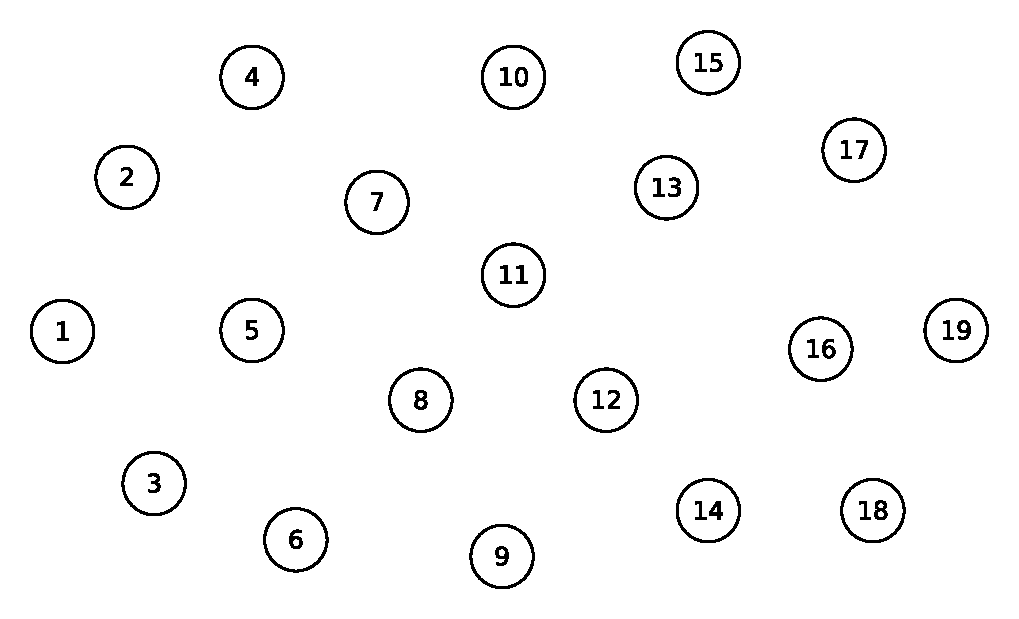
\includegraphics[width=\textwidth]{images/grafo-MTP-1.pdf}
    			\caption{MTP feasible solution}}
    \only<2>{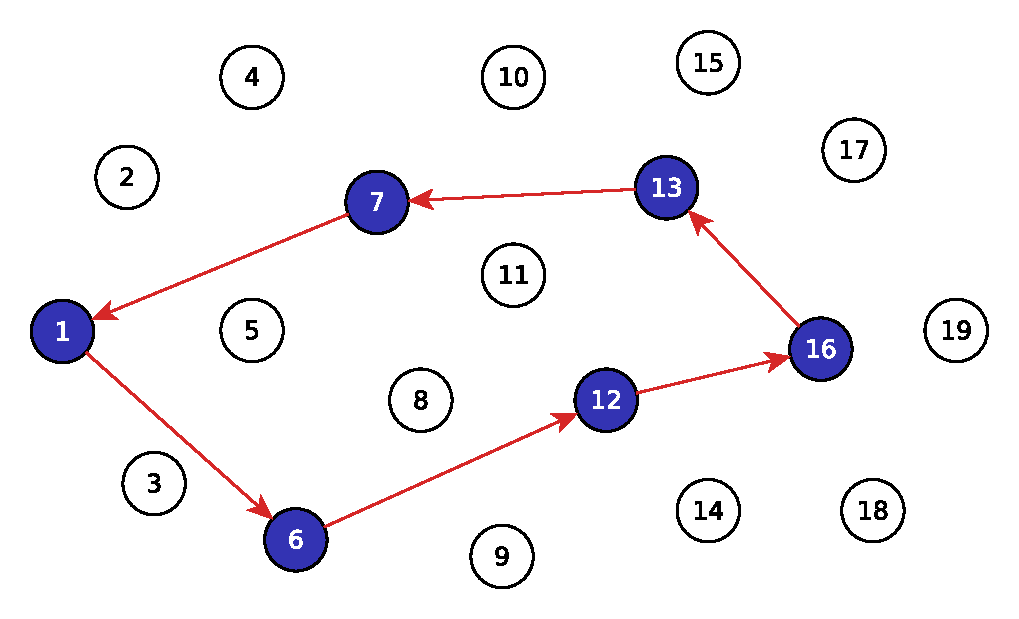
\includegraphics[width=\textwidth]{images/grafo-MTP-2.pdf}
    			\caption{MTP feasible solution}}
    \only<3>{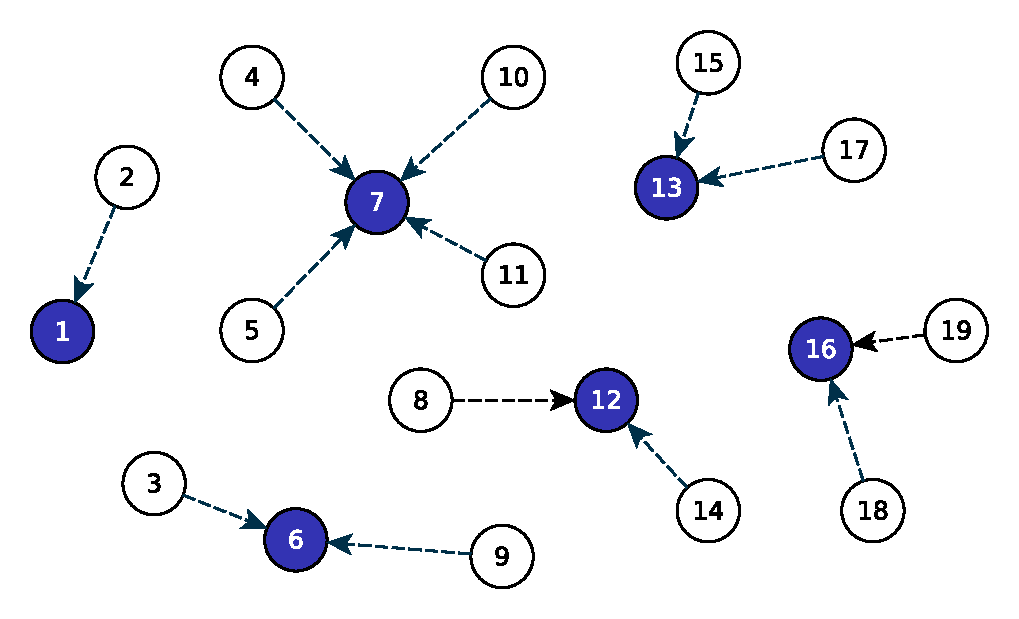
\includegraphics[width=\textwidth]{images/grafo-MTP-3.pdf}
    			\caption{MTP feasible solution}}
    \only<4>{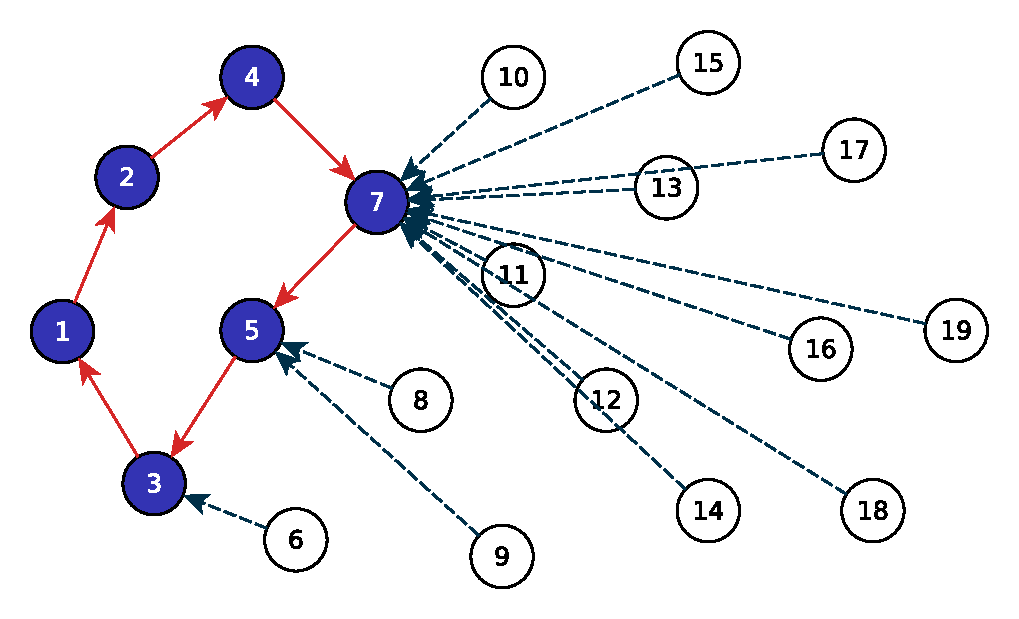
\includegraphics[width=\textwidth]{images/grafo-MTP-Z1.pdf}
    			\caption{MTP feasible solution}}
    \only<5>{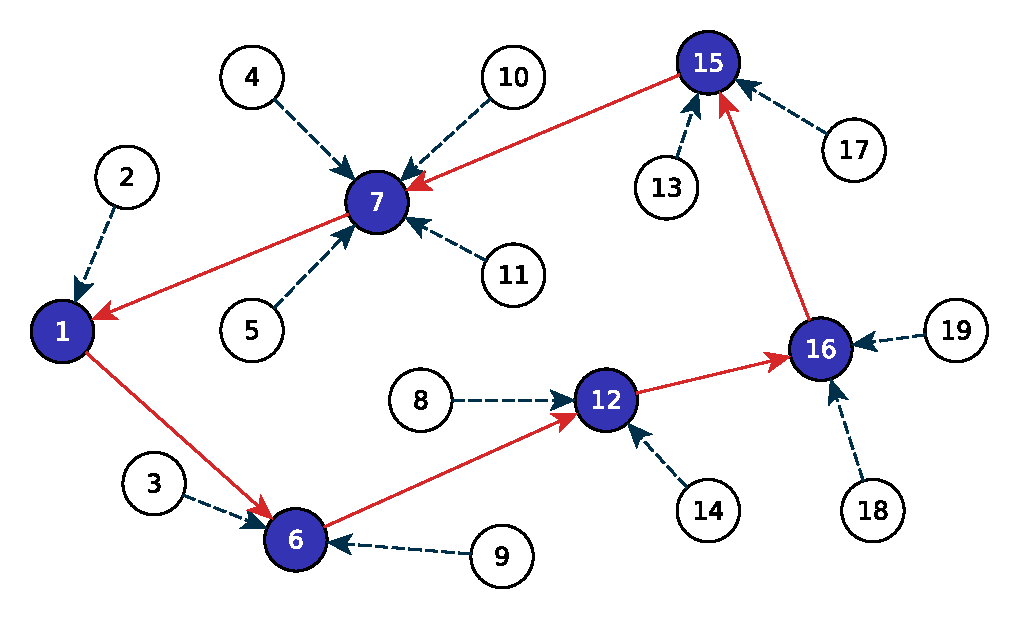
\includegraphics[width=\textwidth]{images/grafo-MTP-Z2.pdf}
    			\caption{MTP feasible solution}}
    \end{figure}
\end{columns}
\end{frame}

\begin{frame}
\frametitle{Research Problem}
\begin{columns}
\column{0.5\textwidth}
We will call \textit{generalized median tour problem} if we combine the \textit{p-median} problem with the \textit{generalized traveling salesman problem}

\column{0.5\textwidth}
    \begin{figure}[ht]
    \centering
    \includegraphics[width=\textwidth]{images/grafo-GMTP-2.pdf}
    \caption{GMTP feasible solution}
    \end{figure}
\end{columns}
\end{frame}


\begin{frame}
\frametitle{Research Problem}
\begin{columns}
\column{0.5\textwidth}
Applications of the problem include:
\begin{itemize}
\item The design of mobile service delivery systems.
\item Bi-modal transportation systems.
\item Distributed computer networks.
\end{itemize}

\column{0.5\textwidth}
    \begin{figure}[ht]
    \centering
    \includegraphics[width=\textwidth]{images/doctors}
    \end{figure}
\end{columns}
\end{frame}


\subsubsection{The Median Tour Problem Generalized with Cumulative Time}
\begin{frame}
\frametitle{Research Problem}
The \textit{median tour problem generalized with cumulative time} is a variation of the \textit{median tour problem}.
\begin{itemize}
\item The GMTPL is a Bi-criterion routing problem.
\item This problem is looking for a balance between the costs of the route and the quality of the service
\item Each node belongs to a cluster.
\item The assignment can only be made between nodes of the same cluster.
\end{itemize}
\end{frame}

\begin{frame}
\frametitle{Research Problem}
\begin{columns}
\column{0.5\textwidth}
	\begin{figure}[ht]
    \centering
    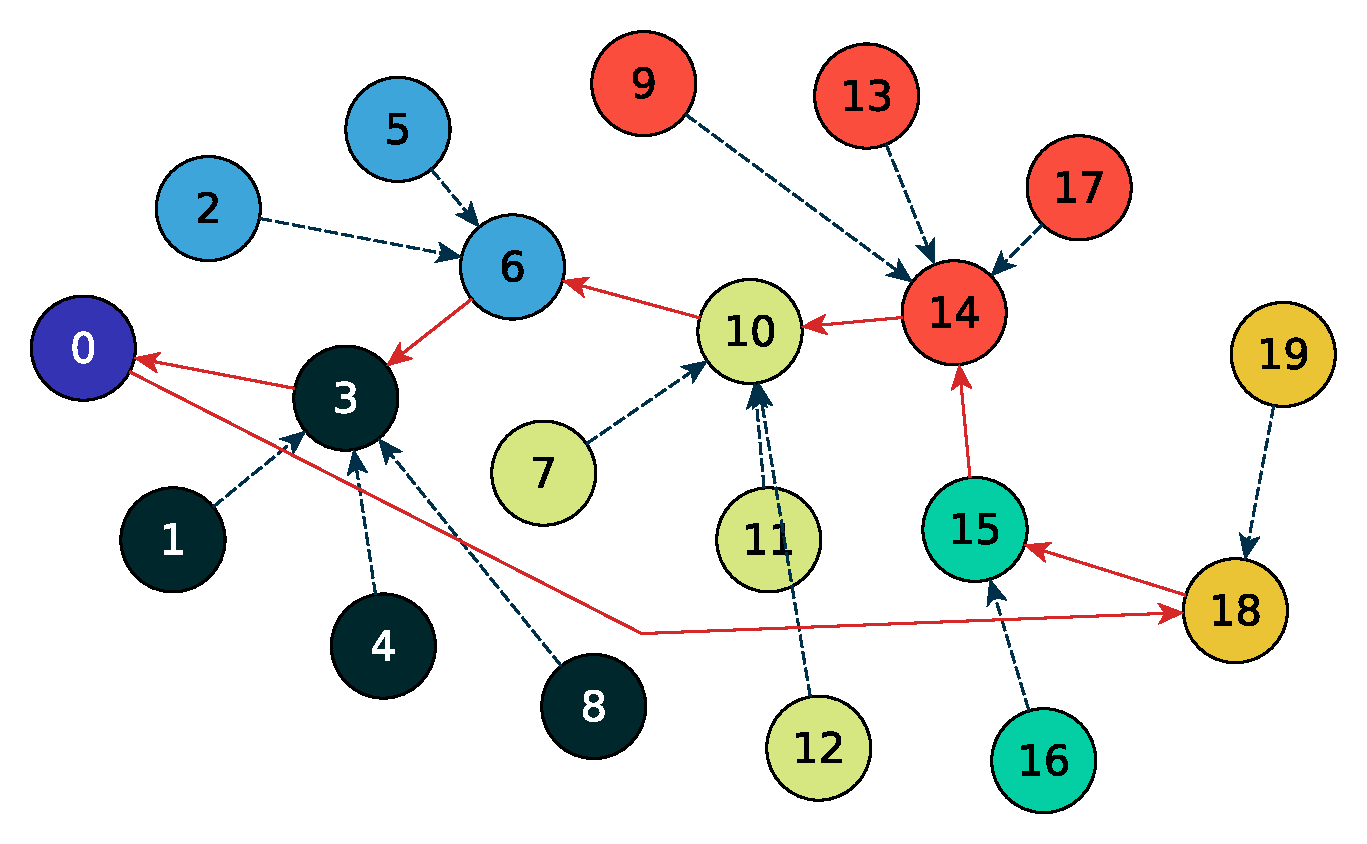
\includegraphics[width=\textwidth]{images/grafo.pdf}
    \caption{GMTPL feasible solution}
    \end{figure}

 
\column{0.5\textwidth}
\begin{definition}
Let $G = (N,A)$ be a complete undirected graph and $V$ a partition of $N$ into $m$ clusters ($V := \set{C_{1}, ..., C_{m}}$ and $C_{i} \cap C_{j} = \emptyset$ for each $i,j \in \set{1,...,m}$). We define the traveling cost $c_{ij}$ and a traveling time $t_{ij}$ associated with each arc $(i,j) \in A$.
\end{definition}
\end{columns}
\end{frame}

\begin{frame}
\frametitle{Research Problem}
\begin{columns}
\column{0.5\textwidth}
	\begin{figure}[ht]
    \centering
    \only<1>{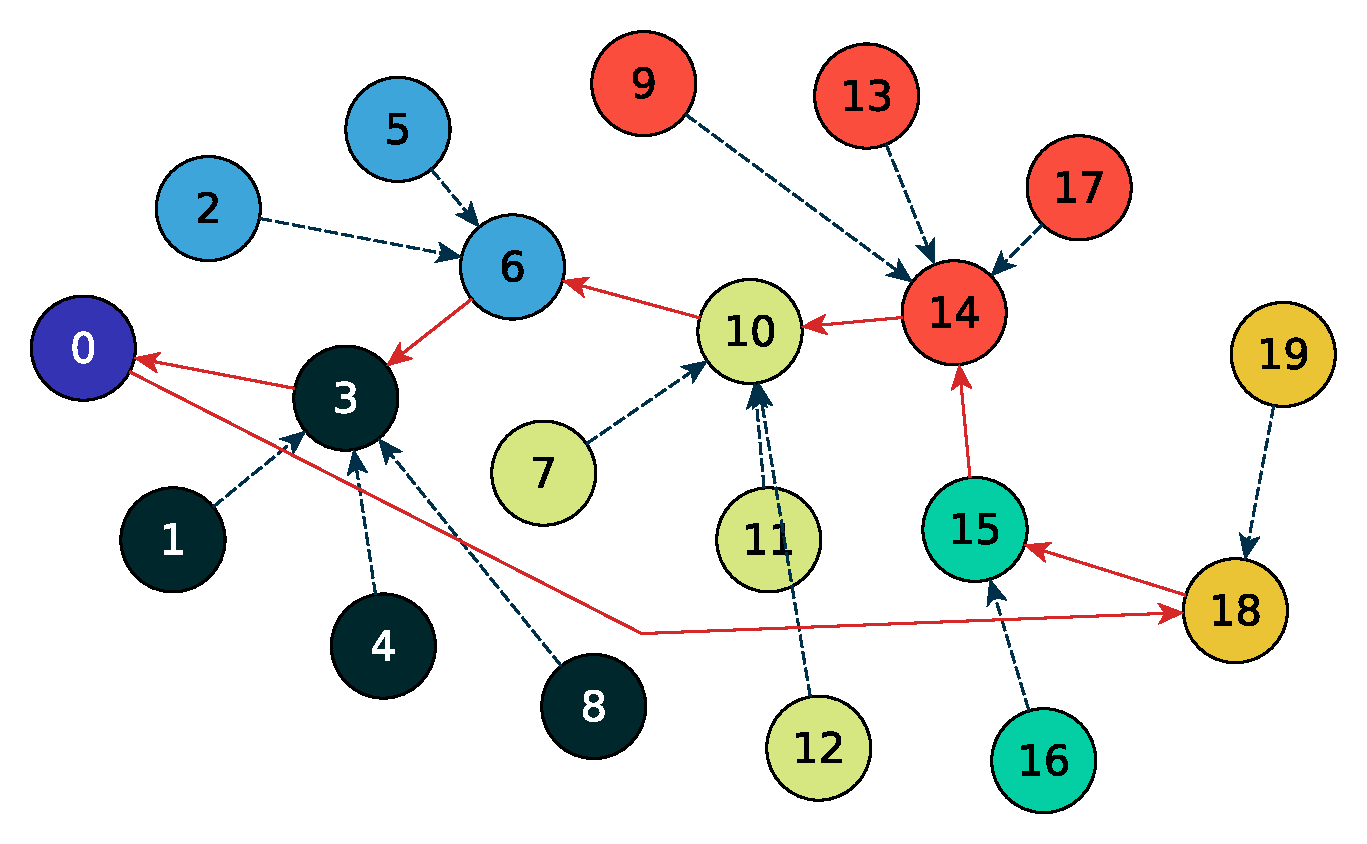
\includegraphics[width=\textwidth]{images/grafo.pdf}
    			\caption{GMTPL feasible solution}}
    \only<2>{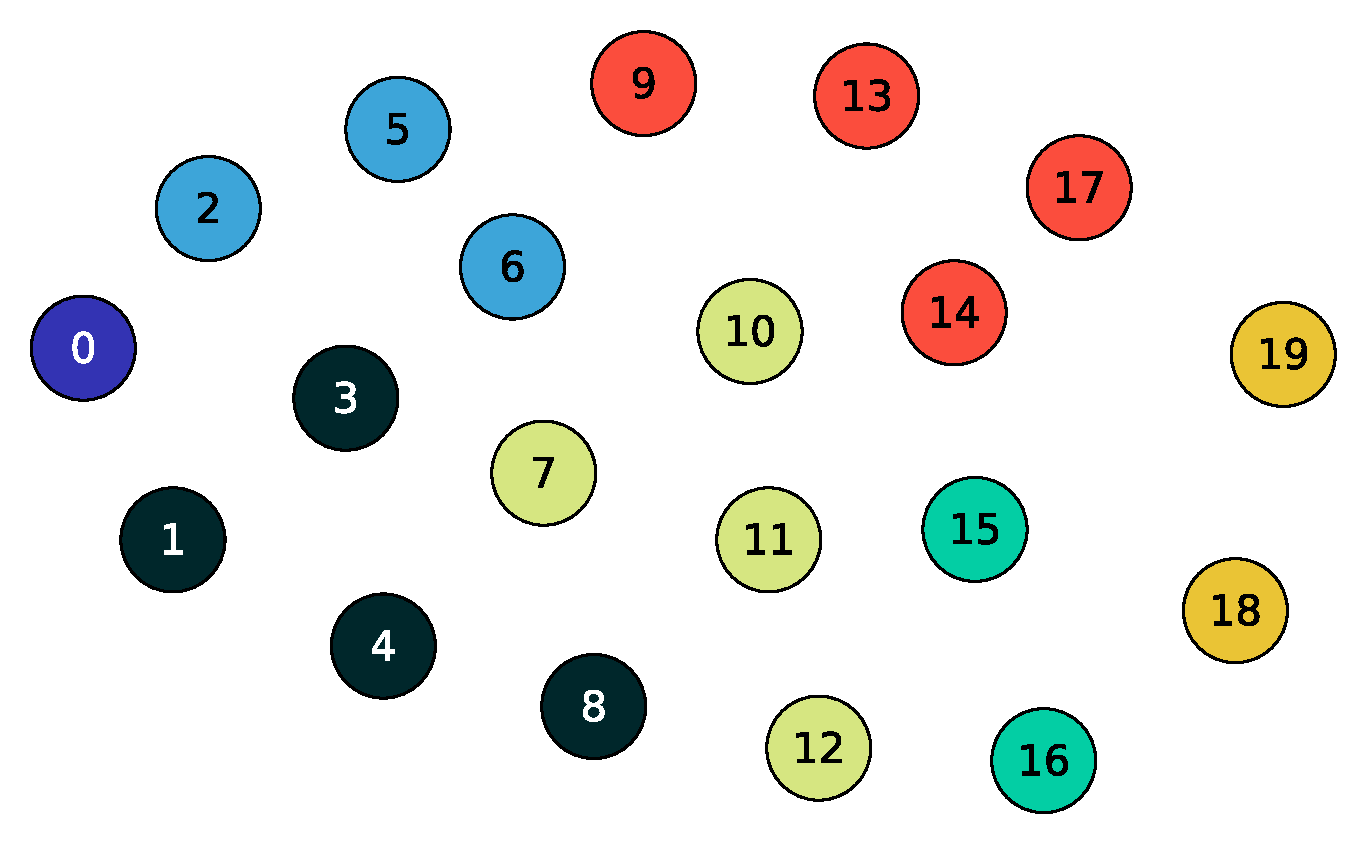
\includegraphics[width=\textwidth]{images/grafo-1.pdf}
    			\caption{GMTPL feasible solution}}
    \only<3>{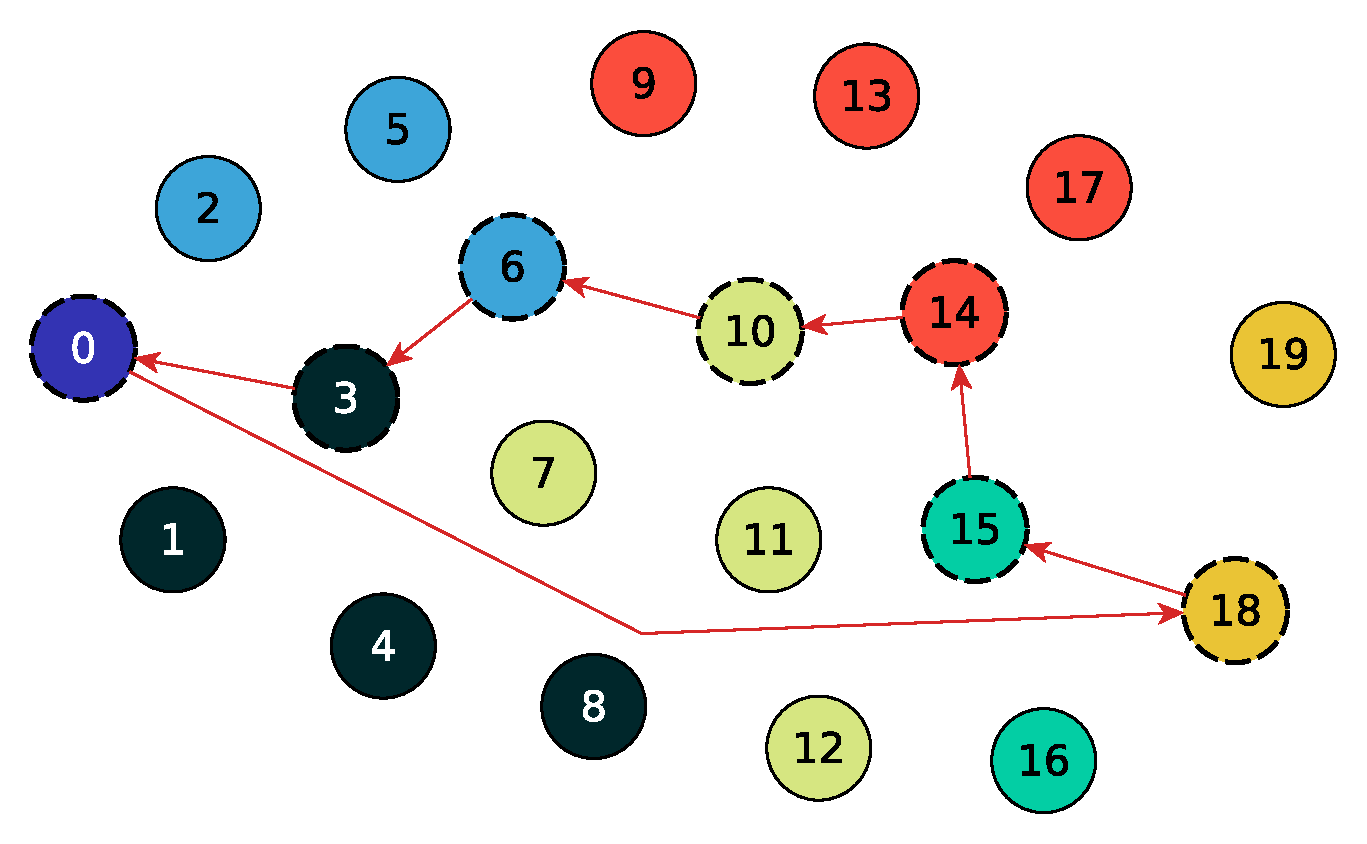
\includegraphics[width=\textwidth]{images/grafo-2.pdf}
    			\caption{GMTPL feasible solution}}
    \only<4>{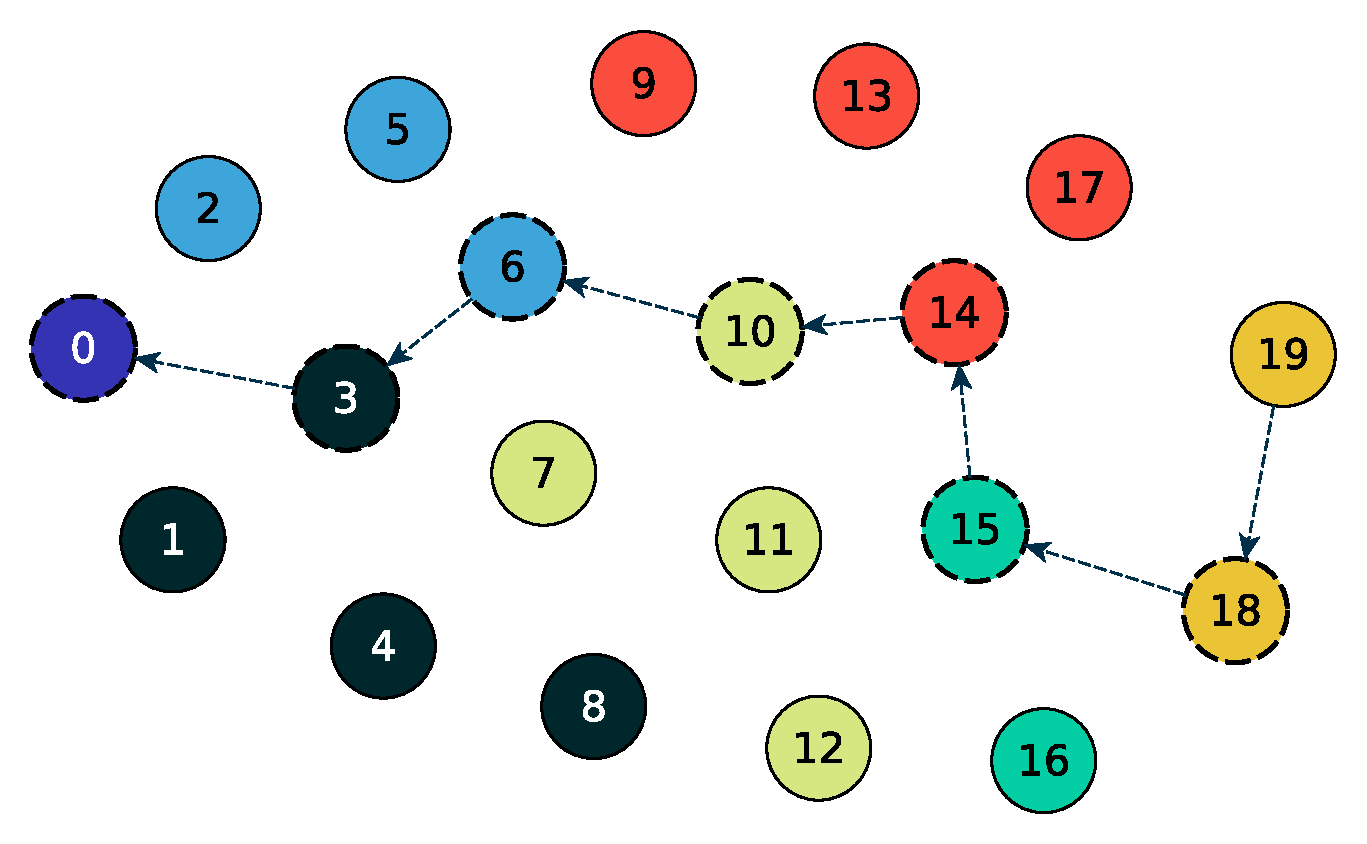
\includegraphics[width=\textwidth]{images/grafo-3.pdf}
    			\caption{GMTPL feasible solution}}
    \end{figure}
\column{0.5\textwidth}
\begin{definition}
The GMTPL consists of finding a route that starts at $0 \in N$ and visits each cluster. The nodes that are not in the tour are assigned to a node of the route within its cluster.

The objective is to minimize the cost associated with the tour and the cumulative time spent on the tour.
\end{definition}
\end{columns}
\end{frame}

\begin{frame}
\frametitle{Research Problem}
\begin{columns}
\column{0.5\textwidth}
MTP applications are maintained.
\begin{itemize}
\item The total time to reach the destination is considered instead of the assignment times
\item It can be used for passenger pick up
\end{itemize}

\column{0.5\textwidth}
    \begin{figure}[ht]
    \centering
    \includegraphics[width=\textwidth]{images/bus}
    \end{figure}
\end{columns}
\end{frame}


{\nologo
\begin{frame}
\frametitle{Research Problem}
\begin{center}
{\large Two cases of the problem will be analyzed:}
\vspace*{\baselineskip}
\end{center}
\begin{columns}
\column{0.5\textwidth}
\begin{block}{Problem 1}
Only one node is visited per cluster and the tour contains $m$ nodes

  \vspace{\baselineskip}
\centering{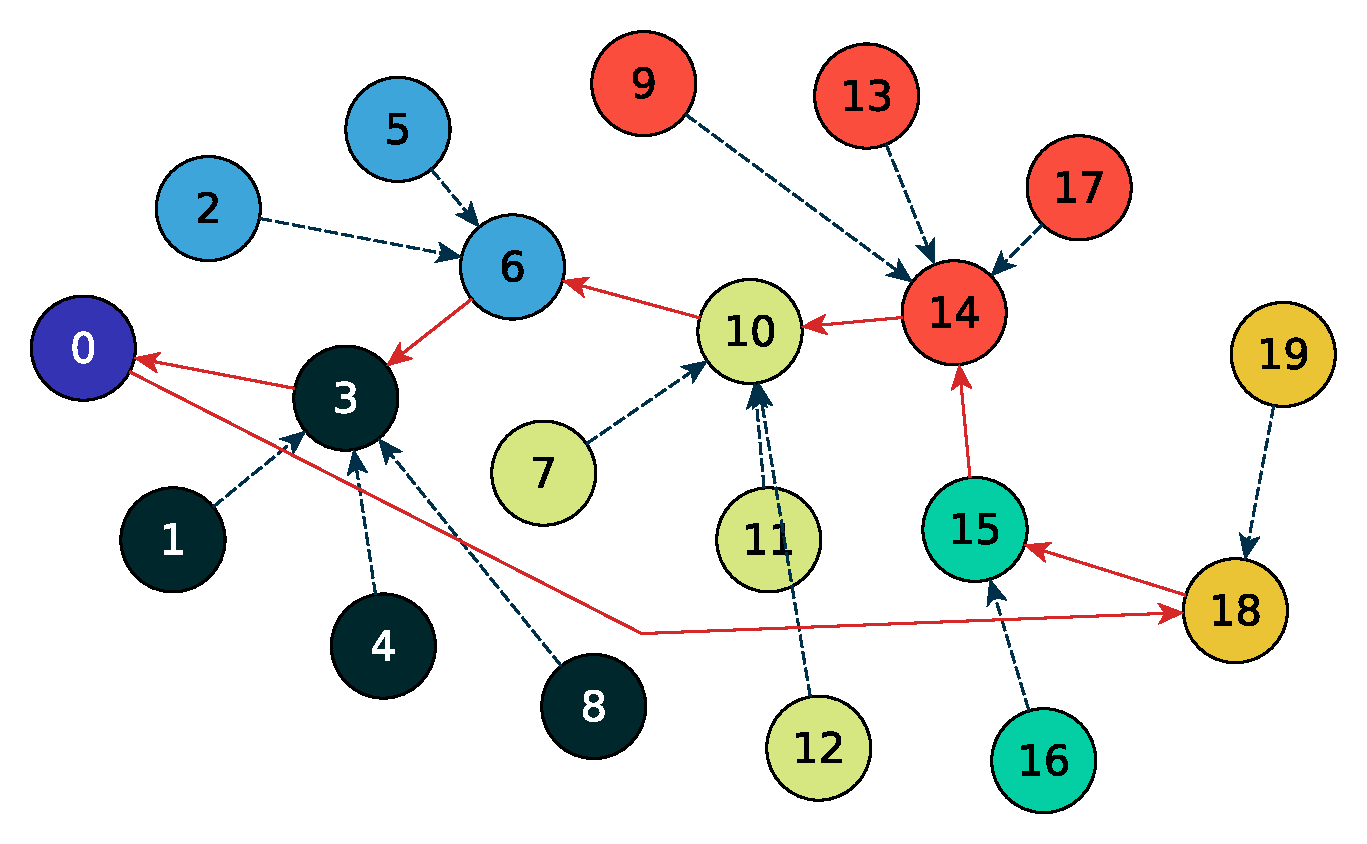
\includegraphics[width=0.6\textwidth]{images/grafo.pdf}}
\end{block}

\column{0.5\textwidth}
\begin{block}{Problem 2}
There are no restrictions regarding the number of tour nodes

  \vspace{\baselineskip}
\centering{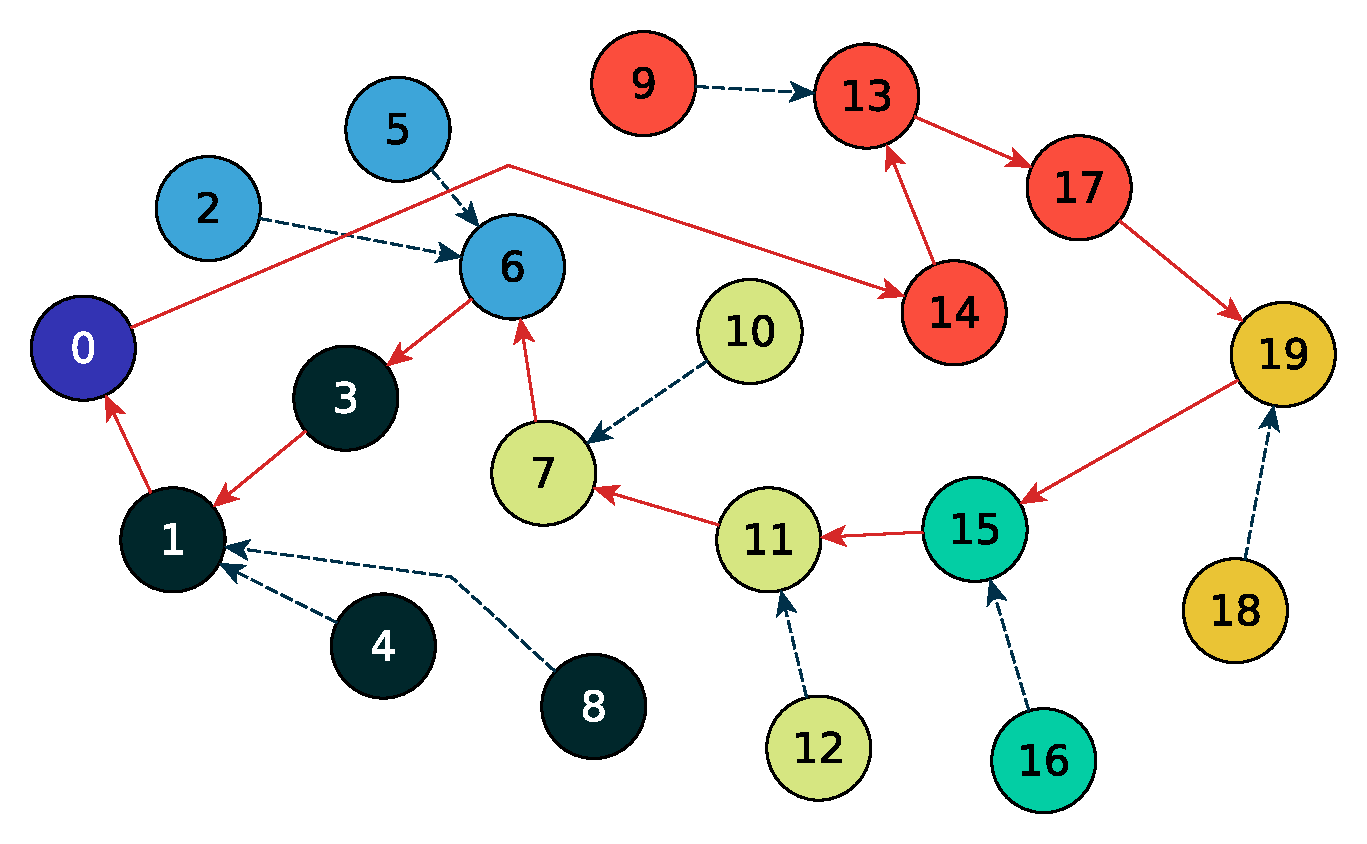
\includegraphics[width=0.6\textwidth]{images/grafo:p2.pdf}}
\end{block}
\end{columns}
\end{frame}
}

\begin{frame}
\frametitle{Research Problem}
\begin{center}
{\large For problem 2, we will define two parameters:}
\end{center}

\begin{definition}
We define the \textit{traveling time 1} ($t_{ij}^1$) and the \textit{traveling time 2} ($t_{ij}^2$) associated with each arc $(i,j) \in A$. The the \textit{traveling time 1} represents the time to reach the tour and the \textit{traveling time 2} is the time on the tour
\end{definition}
\begin{definition}
$t_{ij}^1 \geq t_{ij}^2$ for each arc $(i,j) \in A$
\end{definition}


\end{frame}

\iffalse
\subsection{Objectives}
\begin{frame}
\frametitle{General Objective}
\begin{block}{General Objective}
The general objective is:
\begin{itemize}
\item Apply multi-objective optimization techniques to solve the Median Tour Problem Generalized with Cumulative Time.
\end{itemize}
\end{block}
\end{frame}

\begin{frame}
\frametitle{Specific Objectives}
\begin{block}{Specific Objectives}
The specific objectives are:
\begin{itemize}
\item Propose a mathematical model that allows solving the median tour problem generalized with cumulative time.
\item Design a heuristic that provides solutions efficiently.
\item Generate a set of instances to evaluate the performance of the resolution alternatives.
\end{itemize}
\end{block}
\end{frame}

\fi

\section[Mathematical formulations]{Mathematical formulations}

\begin{frame}
\frametitle{Median Tour Problem Generalized with Cumulative Time}
Before reviewing the mathematical formulations, some sets will be defined
%\vspace*{\baselineskip}
\begin{columns}
\column{0.5\textwidth}
\begin{block}{Definition}
For any $S \subseteq N$, we define $\delta^+(S) := \{(i,j) \in A: i \in S, j \in N\backslash S \}$ and $\delta^-(S) := \{(i,j) \in A: i \in N\backslash S, j \in S\}$. we will use the notation $\delta^+(i)$ and $\delta^+(i)$ when $S = \{i\}$
\end{block}
\column{0.5\textwidth}
     \begin{figure}[ht]
     \centering
     \only<1>{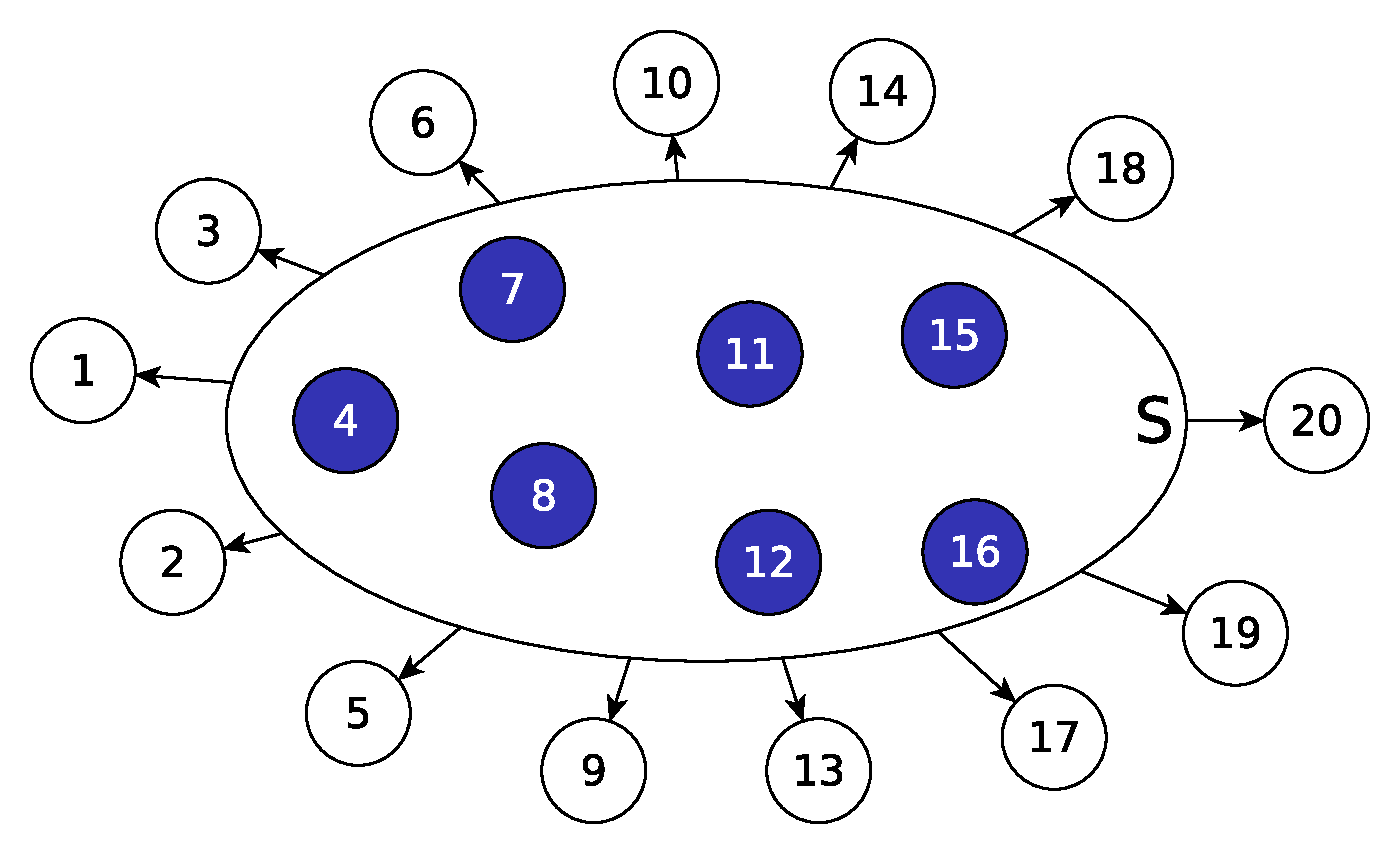
\includegraphics[width=0.9\textwidth]{images/grafo-delta2.pdf}
     			\caption{$\delta^+(S)$}}
     \only<2>{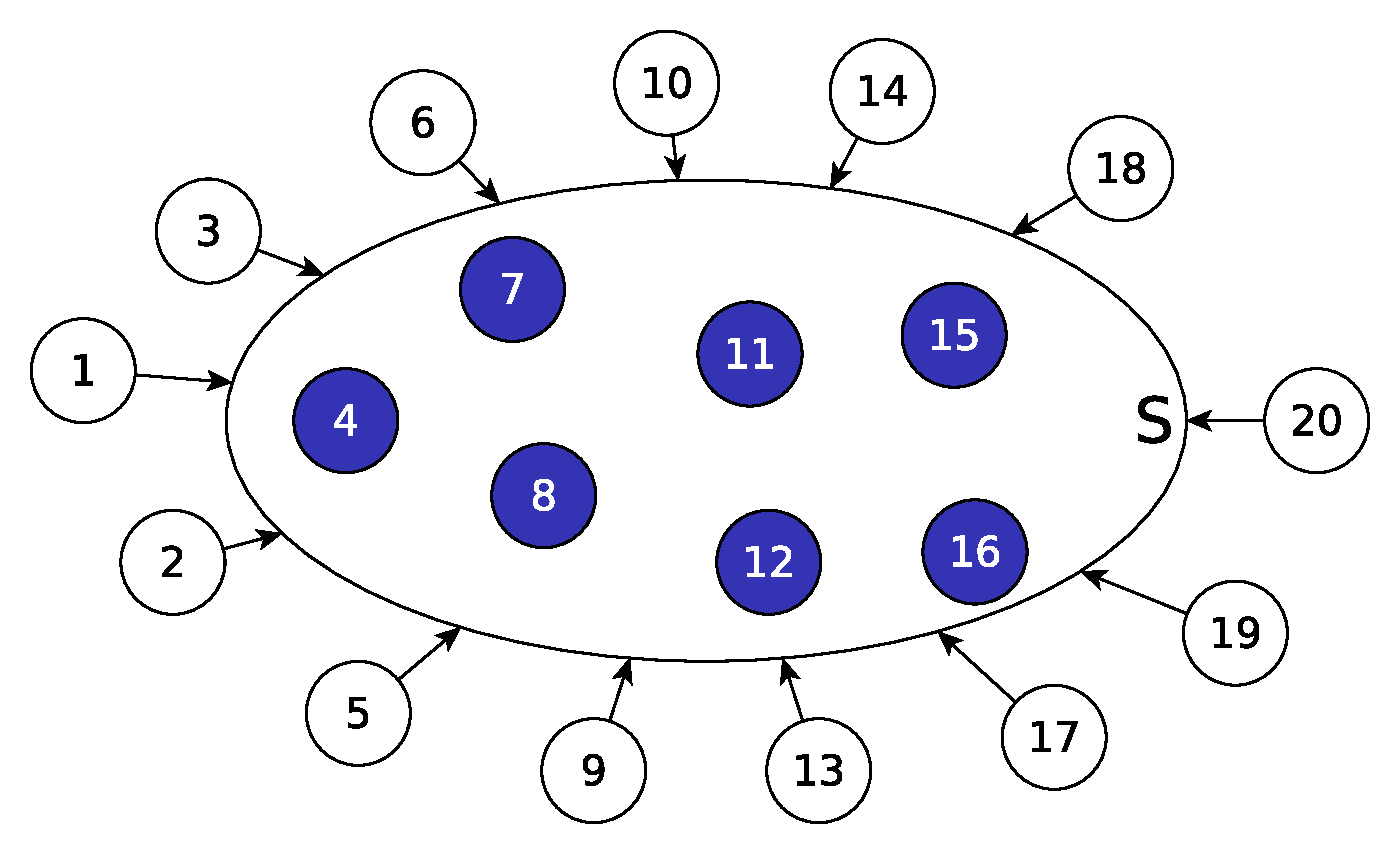
\includegraphics[width=0.9\textwidth]{images/grafo-delta1.pdf}
     			\caption{$\delta^-(S)$ }}
     \end{figure}
\end{columns}
\end{frame}

\iffalse
\begin{frame}
\frametitle{Median Tour Problem Generalized with Cumulative Time}
https://github.com/alexfabianb94/GMTPL/
\end{frame}
\fi

\subsection{Formulations for Problem 1}
\begin{frame}
\frametitle{Problem 1}
  \begin{beamercolorbox}[sep=8pt,center,shadow=true,rounded=true]{title}
    \usebeamerfont{title}{\LARGE Formulations for Problem 1}
  \end{beamercolorbox}
  \vspace{\baselineskip}
\centering{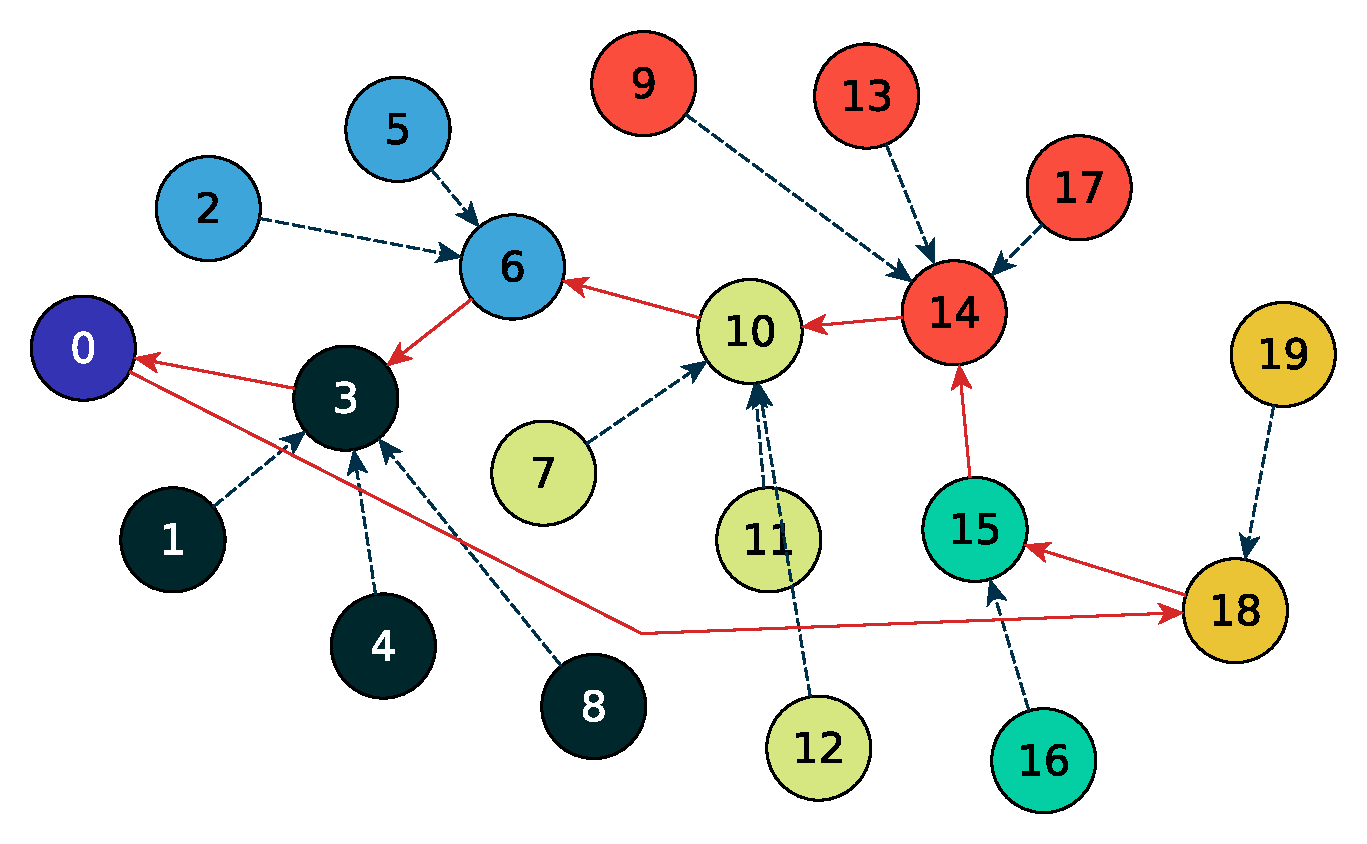
\includegraphics[width=0.4\textwidth]{images/grafo.pdf}}
\end{frame}

\begin{frame}
\frametitle{Formulation 1}
\begin{columns}
\column{0.5\textwidth}
\begin{block}{Formulation 1}
\begin{itemize}
\item It is based on \cite{Fischetti:1993} formulation for the Delivery Man Problem.
\item We use a flow variable that represents the number of times each arc is used.
\end{itemize}
\end{block}
\column{0.5\textwidth}
\begin{block}{Decision Variables}
\[x_{ij}={\begin{cases}1&{\mbox{if the arc $(i,j)$ is used }}\\0&{\mbox{if not}}\end{cases}}
\]
\[y_{ij}={\begin{cases}1&{\mbox{if node i is assigned to node j}}\\0&{\mbox{if not}}\end{cases}}
\]
\[f_{ij} = \mbox{flow from i to j}
\]
\end{block}
\end{columns}
\end{frame}


\iffalse
\begin{frame}
\frametitle{Formulation 1}
\begin{block}{Decision Variables}
\[x_{ij}={\begin{cases}1&{\mbox{if the arc $(i,j)$ is used }}\\0&{\mbox{if not}}\end{cases}}
\]
\[y_{ij}={\begin{cases}1&{\mbox{if node i is assigned to node j}}\\0&{\mbox{if not}}\end{cases}}
\]
\[f_{ij} = \mbox{flow from i to j}
\]
\end{block}
\end{frame}
\fi

\begin{frame}
\frametitle{Formulation 1}
\begin{block}{Objective Function}
\begin{itemize}
\item Total cost of the tour.
\begin{equation*}
Z_1 = \sum_{(i,j) \in A} c_{ij}  x_{ij}
\end{equation*}
\item The cumulative time spent on the tour
\begin{equation*}
Z_2 = \sum_{(i,j) \in A} t_{ij}  f_{ij}
\end{equation*}
\end{itemize}
\end{block}
\end{frame}

\iffalse
\begin{frame}
\frametitle{Formulation 1}
\begin{block}{Constraint}
\begin{footnotesize}
\begin{itemize}
\item Assignment of vertices:
\begin{align}
\label{r1}& \sum_{j \in C_{p}} y_{ij} = 1 & \forall p = 1,...,m; i \in C_{p}\\
\intertext{\item Stops on the tour:}
& y_{jj} = \sum_{(i,j) \in \delta^-(C_{p})} x_{ij}  & \forall p = 1,...,m; j \in C_{p}\\
\intertext{\item Flow conservation:}
& \sum_{(i,j) \in \delta^-(C_{p})} x_{ij} = \sum_{(j,k) \in \delta^+(C_{p})} x_{jk} & \forall p = 1,...,m; j \in C_{p}
\end{align}
\end{itemize}
\end{footnotesize}
\end{block}
\end{frame}

\begin{frame}
\frametitle{Formulation 1}
\begin{block}{Constraint (cont.)}
\begin{footnotesize}
\begin{itemize}
\item Number of Stops:
\begin{align}
& \sum_{(i,j) \in A} x_{ij} = m\\
\intertext{\item Assignment at stops:}
\label{r4}& y_{ij} \leq y_{jj}  & \forall (i,j) \in  A\\
\intertext{\item Vertices flow:}
& \sum_{(i,j) \in A} f_{ij} + 1 = \sum_{(j,k) \in A} f_{jk} & \forall j \in N, j \neq 0
\end{align}
\end{itemize}
\end{footnotesize}
\end{block}
\end{frame}

\begin{frame}
\frametitle{Formulation 1}
\begin{block}{Constraint (cont.)}
\begin{footnotesize}
\begin{itemize}
\item Assignment flow:
\begin{align}
& f_{ij} \leq y_{ij}  & \forall p = 1,...,m; i,j \in C_{p}, i \neq j \\
\intertext{\item Tour flow:}
& f_{ij} \leq |N-1|x_{ij}  & \forall p = 1,...,m;(i,j) \in \delta^+(C_{p})
\end{align}
\end{itemize}
\end{footnotesize}
\end{block}
\end{frame}

\begin{frame}
\frametitle{Formulation 1}
\begin{block}{Constraint (cont.)}
\begin{footnotesize}
\begin{itemize}
\item Variable’s domain:
\begin{align}
& f_{ij} \geq 0 &\forall (i,j) \in A \\
& x_{ij} \in \{0,1\} &\forall (i,j) \in A \\
& y_{ij} \in \{0,1\} &\forall (i,j) \in A
\end{align}
\end{itemize}
\end{footnotesize}
\end{block}
\end{frame}
\fi



\begin{frame}
\frametitle{Formulation 1}
\begin{block}{Constraint}
\begin{scriptsize}
\begin{columns}[t]
\column{0.60\textwidth}
\begin{itemize}
\item Assignment of vertices:
\begin{align}
\label{r1}& \sum_{j \in C_{p}} y_{ij} = 1 & \forall p = 1,...,m; i \in C_{p}\\
\intertext{\item Stops on the tour:}
& y_{jj} = \sum_{(i,j) \in \delta^-(C_{p})} x_{ij}  & \forall p = 1,...,m; j \in C_{p}\\
\intertext{\item Flow conservation:}
& \sum_{(i,j) \in \delta^-(C_{p})} x_{ij} = \sum_{(j,k) \in \delta^+(C_{p})} x_{jk} & \forall p = 1,...,m; j \in C_{p}
\end{align}
\end{itemize}
\column{0.4\textwidth}
\begin{itemize}
\item Number of Stops:
\begin{align}
& \sum_{(i,j) \in A} x_{ij} = m\\
\intertext{\item Assignment at stops:}
\label{r4}& y_{ij} \leq y_{jj}  & \forall (i,j) \in  A
\end{align}
\end{itemize}
\vfill
\end{columns}
\end{scriptsize}
\end{block}
\end{frame}

\begin{frame}
\frametitle{Formulation 1}
\begin{block}{Constraint (cont.)}
\begin{scriptsize}
\begin{columns}[t]
\column{0.61\textwidth}
\begin{itemize}
\item Vertices flow:
\begin{align}
& \sum_{(i,j) \in A} f_{ij} + 1 = \sum_{(j,k) \in A} f_{jk} & \forall j \in N, j \neq 0 \\
\intertext{\item Assignment flow:}
& f_{ij} \leq y_{ij}  & \forall p = 1,...,m; i,j \in C_{p}, i \neq j \\
\intertext{\item Tour flow:}
& f_{ij} \leq |N-1|x_{ij}  & \forall p = 1,...,m;(i,j) \in \delta^+(C_{p})
\end{align}
\end{itemize}
\column{0.39\textwidth}
\begin{itemize}
\item Variable’s domain:
\begin{align}
& f_{ij} \geq 0 &\forall (i,j) \in A \\
& x_{ij} \in \{0,1\} &\forall (i,j) \in A \\
& y_{ij} \in \{0,1\} &\forall (i,j) \in A
\end{align}
\end{itemize}
\end{columns}
\end{scriptsize}
\end{block}
\end{frame}



\begin{frame}
\frametitle{Formulation 2}
\begin{columns}
\column{0.4\textwidth}
\begin{block}{Formulation 2}
\begin{itemize}
\item Based on multicommodity flow formulation.
\item Requires at least $|N|^3$ variables.
\end{itemize}
\end{block}
\column{0.6\textwidth}
\begin{block}{Decision Variables}
\[x_{ij}={\begin{cases}1&{\mbox{if the arc $(i,j)$ is used }}\\0&{\mbox{if not}}\end{cases}}
\]
\[y_{ij}={\begin{cases}1&{\mbox{if node $i$ is assigned to node $j$}}\\0&{\mbox{if not}}\end{cases}}
\]
\[f_{ij}^k = \mbox{flow through the arc $(i,j)$, originating in node $k$}
\]
\end{block}
\end{columns}
\end{frame}

\iffalse
\begin{frame}
\frametitle{Formulation 2}
\begin{block}{Decision Variables}
\[x_{ij}={\begin{cases}1&{\mbox{if the arc $(i,j)$ is used }}\\0&{\mbox{if not}}\end{cases}}
\]
\[y_{ij}={\begin{cases}1&{\mbox{if node $i$ is assigned to node $j$}}\\0&{\mbox{if not}}\end{cases}}
\]
\[f_{ij}^k = \mbox{flow through the arc $(i,j)$, originating in node $k$}
\]
\end{block}
\end{frame}
\fi

\begin{frame}
\frametitle{Formulation 2}
\begin{block}{Objective Function}
\begin{itemize}
\item Total cost of the tour.
\begin{equation*}
Z_1 = \sum_{(i,j) \in A} c_{ij}  x_{ij}
\end{equation*}
\item The cumulative time spent on the tour
\begin{equation*}
Z_2 = \sum_{k \in N}\sum_{(i,j) \in A} t_{ij} f_{ij}^k
\end{equation*}
\end{itemize}
\end{block}
\end{frame}

\iffalse
\begin{frame}
\frametitle{Formulation 2}
\begin{block}{Constraint}
\begin{footnotesize}
\begin{itemize}
\item[]
\begin{align}
&(\ref{r1}) - (\ref{r4}) \nonumber \\
\intertext{\item Flow conservation:}
& \sum_{(i,j) \in A: i \neq 0} f_{ij}^k = \sum_{(j,h) \in A} f_{jh}^k & \forall j, k \in N \backslash\{0\}, j \neq k\\
\intertext{\item Flow source:}
& \sum_{(k,j) \in A} f_{kj}^k = 1 & \forall k \in N \backslash\{0\}
\end{align}
\end{itemize}
\end{footnotesize}
\end{block}
\end{frame}

\begin{frame}
\frametitle{Formulation 2}
\begin{block}{Constraint (cont.)}
\begin{footnotesize}
\begin{itemize}
\item Flow destination:
\begin{align}
& \sum_{(i,0) \in A} f_{i0}^k = 1 & \forall k \in N \backslash\{0\}\\
\intertext{\item Assignment flow:}
& f_{ij}^k \leq y_{ij}  & \forall p = 1,...,m; i,j,k \in C_{p}, i \neq j
\intertext{\item Tour flow:}
& f_{ij}^k \leq x_{ij}  & \forall p = 1,...,m; i \in N, j \in N \backslash C_{p}, k \in C_{p}
\end{align}
\end{itemize}
\end{footnotesize}
\end{block}
\end{frame}

\begin{frame}
\frametitle{Formulation 2}
\begin{block}{Constraint (cont.)}
\begin{footnotesize}
\begin{itemize}
\item Variable’s domain:
\begin{align}
& f_{ij}^k \geq 0 &\forall (i,j) \in A, k \in N \\
& x_{ij} \in \{0,1\} &\forall (i,j) \in A \\
& y_{ij} \in \{0,1\} &\forall (i,j) \in A
\end{align}
\end{itemize}
\end{footnotesize}
\end{block}
\end{frame}
\fi

\begin{frame}
\frametitle{Formulation 2}
\begin{block}{Constraint}
\begin{scriptsize}
\centering {(\ref{r1}) - (\ref{r4})}
\begin{itemize}
\item Flow conservation:
\begin{align}
& \sum_{(i,j) \in A: i \neq 0} f_{ij}^k = \sum_{(j,h) \in A} f_{jh}^k & \forall j, k \in N \backslash\{0\}, j \neq k\\
\intertext{\item Assignment flow:}
& f_{ij}^k \leq y_{ij}  & \forall p = 1,...,m; i,j,k \in C_{p}, i \neq j \\
\intertext{\item Tour flow:}
& f_{ij}^k \leq x_{ij}  & \forall p = 1,...,m; i \in N, j \in N \backslash C_{p}, k \in C_{p}
\end{align}
\end{itemize}
\end{scriptsize}
\end{block}
\end{frame}

\begin{frame}
\frametitle{Formulation 2}
\begin{block}{Constraint (cont.)}
\begin{footnotesize}
\begin{columns}[t]
\column{0.5\textwidth}
\begin{itemize}
\item Flow source:
\begin{align}
& \sum_{(k,j) \in A} f_{kj}^k = 1 & \forall k \in N \backslash\{0\} \\
\intertext{\item Flow destination:}
& \sum_{(i,0) \in A} f_{i0}^k = 1 & \forall k \in N \backslash\{0\}
\end{align}
\end{itemize}
\column{0.5\textwidth}
\begin{itemize}
\item Variable’s domain:
\begin{align}
& f_{ij}^k \geq 0 &\forall (i,j) \in A, k \in N \\
& x_{ij} \in \{0,1\} &\forall (i,j) \in A \\
& y_{ij} \in \{0,1\} &\forall (i,j) \in A
\end{align}
\end{itemize}
\end{columns}
\end{footnotesize}
\end{block}
\end{frame}


\begin{frame}
\frametitle{Formulation 3}
\begin{columns}
\column{0.5\textwidth}
\begin{block}{Formulation 3}
\begin{itemize}
\item The MTZ restriction determine the cumulative time.
\item The linear relaxation of the problem is of lower quality.
\end{itemize}
\end{block}
\column{0.5\textwidth}
\begin{block}{Decision Variables}
\[x_{ij}={\begin{cases}1&{\mbox{if the arc $(i,j)$ is used }}\\0&{\mbox{if not}}\end{cases}}
\]
\[y_{ij}={\begin{cases}1&{\mbox{if node $i$ is assigned to node $j$}}\\0&{\mbox{if not}}\end{cases}}
\]
\[u_{j} = \mbox{cumulative time of node $j$}
\]
\end{block}

\end{columns}
\end{frame}

\iffalse
\begin{frame}
\frametitle{Formulation 3}
\begin{block}{Decision Variables}
\[x_{ij}={\begin{cases}1&{\mbox{if the arc $(i,j)$ is used }}\\0&{\mbox{if not}}\end{cases}}
\]
\[y_{ij}={\begin{cases}1&{\mbox{if node $i$ is assigned to node $j$}}\\0&{\mbox{if not}}\end{cases}}
\]
\[u_{j} = \mbox{cumulative time of node $j$}
\]
\end{block}
\end{frame}
\fi

\begin{frame}
\frametitle{Formulation 3}
\begin{block}{Objective Function}
\begin{itemize}
\item Total cost of the tour.
\begin{equation*}
Z_1 = \sum_{(i,j) \in A} c_{ij}  x_{ij}
\end{equation*}
\item The cumulative time spent on the tour
\begin{equation*}
Z_2 = \sum_{j \in N} u_j
\end{equation*}
\end{itemize}
\end{block}
\end{frame}

\iffalse
\begin{frame}
\frametitle{Formulation 3}
\begin{block}{Constraint}
\begin{footnotesize}
\begin{itemize}
\item[]
\begin{align}
&(\ref{r1}) - (\ref{r4}) \nonumber \\
\intertext{\item Deposit time:}
& u_0 = 0 \\
\intertext{\item MTZ with cumulative time:}
& u_i \geq u_j + t_{ij} - M (1 - x_{ij} - y_{ij}) & \forall (i,j) \in A, i \neq 0
\end{align}
\end{itemize}
\end{footnotesize}
\end{block}
\end{frame}

\begin{frame}
\frametitle{Formulation 3}
\begin{block}{Constraint (cont.)}
\begin{footnotesize}
\begin{itemize}
\item Variable’s domain:
\begin{align}
& u_{j} \geq 0 &\forall j \in N \\
& x_{ij} \in \{0,1\} &\forall (i,j) \in A \\
& y_{ij} \in \{0,1\} &\forall (i,j) \in A
\end{align}
\end{itemize}
\end{footnotesize}
\end{block}
\end{frame}
\fi



\begin{frame}
\frametitle{Formulation 3}
\begin{block}{Constraint}
\begin{scriptsize}
\begin{columns}[t]
\column{0.6\textwidth}
\centering {(\ref{r1}) - (\ref{r4})}
\begin{itemize}
\item Deposit time:
\begin{align}
& u_0 = 0 \\
\intertext{\item MTZ with cumulative time:}
& u_i \geq u_j + t_{ij} - M (1 - x_{ij} - y_{ij}) & \forall (i,j) \in A, i \neq 0
\end{align}
\end{itemize}
\column{0.4\textwidth}
\begin{itemize}
\item Variable’s domain:
\begin{align}
& u_{j} \geq 0 &\forall j \in N \\
& x_{ij} \in \{0,1\} &\forall (i,j) \in A \\
& y_{ij} \in \{0,1\} &\forall (i,j) \in A
\end{align}
\end{itemize}
\end{columns}
\end{scriptsize}
\end{block}
\end{frame}



\subsection{Formulations for Problem 2}
\begin{frame}
\frametitle{Problem 2}
  \begin{beamercolorbox}[sep=8pt,center,shadow=true,rounded=true]{title}
    \usebeamerfont{title}{\LARGE Formulations for Problem 2}
  \end{beamercolorbox}
  \vspace{\baselineskip}
\centering{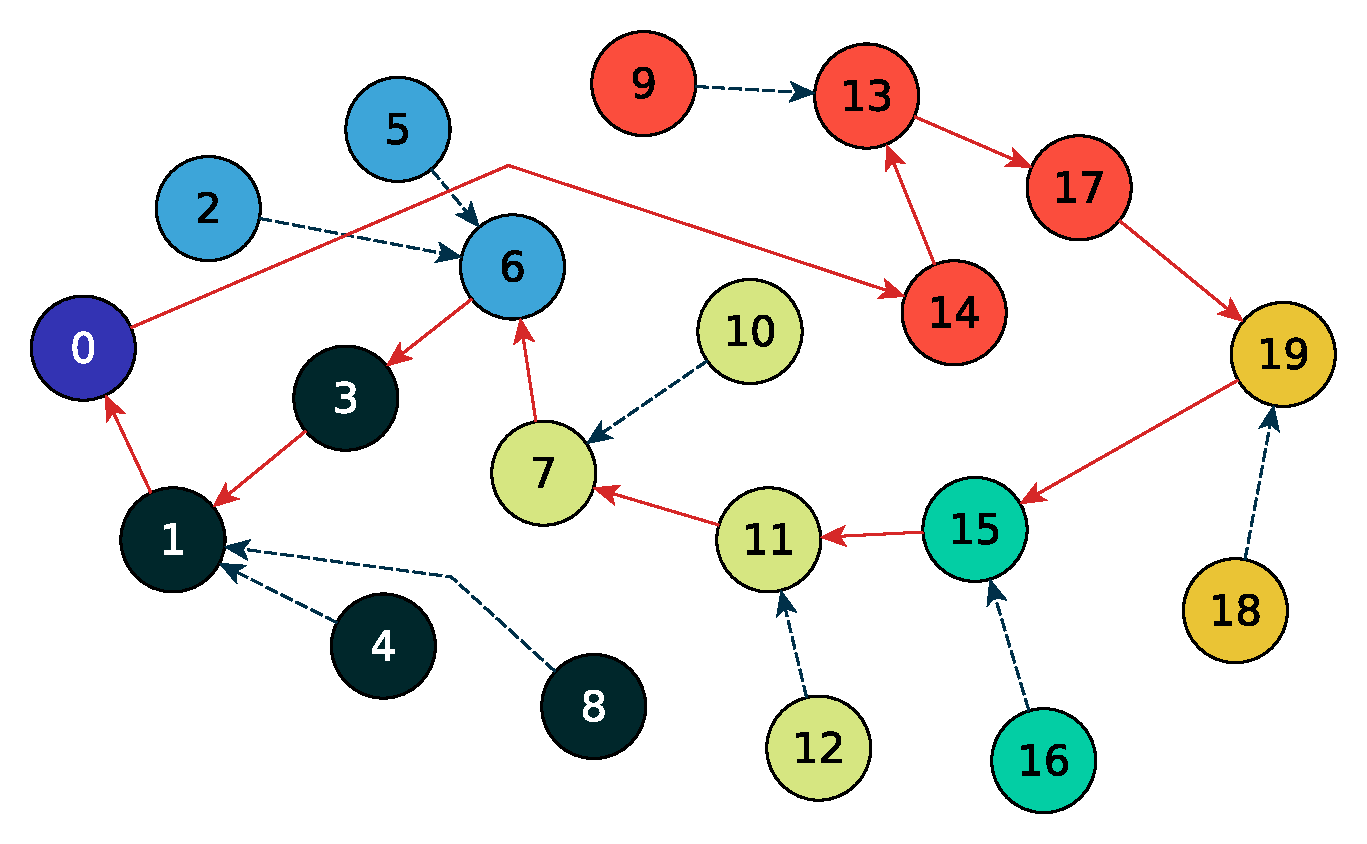
\includegraphics[width=0.4\textwidth]{images/grafo:p2.pdf}}
\end{frame}


\begin{frame}
\frametitle{Formulation 4}
\begin{columns}
\column{0.5\textwidth}
\begin{block}{Formulation 4}
\begin{itemize}
\item It is based on the formulation 3.
\item It is allowed to visit more than one node per cluster.
\
\end{itemize}
\end{block}
\column{0.5\textwidth}
\begin{block}{Decision Variables}
\[x_{ij}={\begin{cases}1&{\mbox{if the arc $(i,j)$ is used }}\\0&{\mbox{if not}}\end{cases}}
\]
\[y_{ij}={\begin{cases}1&{\mbox{if node $i$ is assigned to node $j$}}\\0&{\mbox{if not}}\end{cases}}
\]
\[u_{j} = \mbox{cumulative time of node $j$}
\]
\end{block}
\end{columns}
\end{frame}

\iffalse
\begin{frame}
\frametitle{Formulation 4}
\begin{block}{Decision Variables}
\[x_{ij}={\begin{cases}1&{\mbox{if the arc $(i,j)$ is used }}\\0&{\mbox{if not}}\end{cases}}
\]
\[y_{ij}={\begin{cases}1&{\mbox{if node $i$ is assigned to node $j$}}\\0&{\mbox{if not}}\end{cases}}
\]
\[u_{j} = \mbox{cumulative time of node $j$}
\]
\end{block}
\end{frame}
\fi


\begin{frame}
\frametitle{Formulation 4}
\begin{block}{Objective Function}
\begin{itemize}
\item Total cost of the tour.
\begin{equation*}
Z_1 = \sum_{(i,j) \in A} c_{ij}  x_{ij}
\end{equation*}
\item The cumulative time spent on the tour
\begin{equation*}
Z_2 = \sum_{j \in N} u_j
\end{equation*}
\end{itemize}
\end{block}
\end{frame}

\iffalse
\begin{frame}
\frametitle{Formulation 4}
\begin{block}{Constraint}
\begin{footnotesize}
\begin{itemize}
\item Assignment of vertices:
\begin{align}
\label{r5}& \sum_{j \in C_{p}} y_{ij} = 1 & \forall p = 1,...,m; i \in C_{p}\\
\intertext{\item Stops on the tour:}
& y_{jj} = \sum_{(i,j) \in A} x_{ij}  & \forall j \in N\\
\intertext{\item Flow conservation:}
& \sum_{(i,j) \in A} x_{ij} = \sum_{(j,k) \in A} x_{jk} & \forall j \in N
\end{align}
\end{itemize}
\end{footnotesize}
\end{block}
\end{frame}

\begin{frame}
\frametitle{Formulation 4}
\begin{block}{Constraint (cont.)}
\begin{footnotesize}
\begin{itemize}
\item Assignment at stops:
\begin{align}
\label{r6}& y_{ij} \leq y_{jj}  & \forall (i,j) \in  A \\
\intertext{\item Deposit time:}
& u_0 = 0 \\
\intertext{\item MTZ with cumulative time:}
& u_i \geq u_j + t_{ij}^1 y_{ij} + t_{ij}^2 x_{ij} - M (1 - x_{ij} - y_{ij}) & \forall (i,j) \in A, i \neq 0
\end{align}
\end{itemize}
\end{footnotesize}
\end{block}
\end{frame}

\begin{frame}
\frametitle{Formulation 4}
\begin{block}{Constraint (cont.)}
\begin{footnotesize}
\begin{itemize}
\item Variable’s domain:
\begin{align}
& u_{j} \geq 0 &\forall j \in N \\
& x_{ij} \in \{0,1\} &\forall (i,j) \in A \\
& y_{ij} \in \{0,1\} &\forall (i,j) \in A
\end{align}
\end{itemize}
\end{footnotesize}
\end{block}
\end{frame}
\fi


\begin{frame}
\frametitle{Formulation 4}
\begin{block}{Constraint}
\begin{scriptsize}
\begin{columns}[t]
\column{0.55\textwidth}
\begin{itemize}
\item Assignment of vertices:
\begin{align}
\label{r5}& \sum_{j \in C_{p}} y_{ij} = 1 & \forall p = 1,...,m; i \in C_{p}\\
\intertext{\item Stops on the tour:}
& y_{jj} = \sum_{(i,j) \in A} x_{ij}  & \forall j \in N\\
\intertext{\item Flow conservation:}
& \sum_{(i,j) \in A} x_{ij} = \sum_{(j,k) \in A} x_{jk} & \forall j \in N
\end{align}
\end{itemize}
\column{0.45\textwidth}
\begin{itemize}
\item Incidence arcs to the cluster:
\begin{align}
& \sum_{(i,j) \in \delta^-(C_{p})} x_{ij} = 1 & \forall p = 1,...,m\\
\intertext{\item Assignment at stops}
\label{r6}& y_{ij} \leq y_{jj}  & \forall (i,j) \in  A \\
\intertext{\item Deposit time:}
& u_0 = 0
\end{align}
\end{itemize}
\end{columns}
\end{scriptsize}
\end{block}
\end{frame}

\begin{frame}
\frametitle{Formulation 4}
\begin{block}{Constraint (cont.)}
\begin{footnotesize}
\begin{itemize}
\item MTZ with cumulative time:
\begin{align}
& u_i \geq u_j + t_{ij}^1 y_{ij} + t_{ij}^2 x_{ij} - M (1 - x_{ij} - y_{ij}) & \forall (i,j) \in A, i \neq 0 \\
\intertext{\item Variable’s domain:}
& u_{j} \geq 0 &\forall j \in N \\
& x_{ij} \in \{0,1\} &\forall (i,j) \in A \\
& y_{ij} \in \{0,1\} &\forall (i,j) \in A
\end{align}
\end{itemize}
\end{footnotesize}
\end{block}
\end{frame}

\begin{frame}
\frametitle{Formulation 5}
\begin{columns}
\column{0.4\textwidth}
\begin{block}{Formulation 5}
\begin{itemize}
\item It is based on the formulation 2.
\item It is allowed to visit more than one node per cluster
\end{itemize}
\end{block}
\column{0.6\textwidth}
\begin{block}{Decision Variables}
\[x_{ij}={\begin{cases}1&{\mbox{if the arc $(i,j)$ is used }}\\0&{\mbox{if not}}\end{cases}}
\]
\[y_{ij}={\begin{cases}1&{\mbox{if node $i$ is assigned to node $j$}}\\0&{\mbox{if not}}\end{cases}}
\]
\[f_{ij}^k = \mbox{flow through the arc $(i,j)$, originating in node $k$}
\]
\end{block}
\end{columns}
\end{frame}

\iffalse
\begin{frame}
\frametitle{Formulation 5}
\begin{block}{Decision Variables}
\[x_{ij}={\begin{cases}1&{\mbox{if the arc $(i,j)$ is used }}\\0&{\mbox{if not}}\end{cases}}
\]
\[y_{ij}={\begin{cases}1&{\mbox{if node $i$ is assigned to node $j$}}\\0&{\mbox{if not}}\end{cases}}
\]
\[f_{ij}^k = \mbox{flow through the arc $(i,j)$, originating in node $k$}
\]
\end{block}
\end{frame}
\fi

\begin{frame}
\frametitle{Formulation 5}
\begin{block}{Objective Function}
\begin{itemize}
\item Total cost of the tour.
\begin{equation*}
Z_1 = \sum_{(i,j) \in A} c_{ij}  x_{ij}
\end{equation*}
\item The cumulative time spent on the tour
\begin{equation*}
Z_2 = \sum_{(i,j) \in A} t_{ij}^1 y_{ij} + \sum_{k \in N}\sum_{(i,j) \in A: i \neq k} t_{ij}^2  f_{ij}^k + \sum_{p = 1}^{m} \sum_{(k,j) \in \delta^+(C_{p})} t_{kj}^2 f_{kj}^k + \sum_{p = 1}^{m} \sum_{i,j \in C_p: i \neq j} t_{ij}^2 x_{ij} 
\end{equation*}
\end{itemize}
\end{block}
\end{frame}



\iffalse
\begin{frame}
\frametitle{Formulation 5}
\begin{block}{Constraint}
\begin{footnotesize}
\begin{itemize}
\item[]
\begin{align}
&(\ref{r5}) - (\ref{r6}) \nonumber \\
\intertext{\item Flow conservation:}
& \sum_{(i,j) \in A: i \neq 0} f_{ij}^k = \sum_{(j,h) \in A} f_{jh}^k & \forall j, k \in N \backslash\{0\}, j \neq k\\
\intertext{\item Flow source:}
& \sum_{(k,j) \in A} f_{kj}^k = 1 & \forall k \in N \backslash\{0\}
\end{align}
\end{itemize}
\end{footnotesize}
\end{block}
\end{frame}

\begin{frame}
\frametitle{Formulation 5}
\begin{block}{Constraint (cont.)}
\begin{footnotesize}
\begin{itemize}
\item Flow destination:
\begin{align}
& \sum_{(i,0) \in A} f_{i0}^k = 1 & \forall k \in N \backslash\{0\}\\
\intertext{\item Assignment flow:}
& f_{kj}^k \leq y_{kj}  & \forall p = 1,...,m; k,j \in C_{p}, i \neq j\\
\intertext{\item Tour flow 1:}
& f_{ij}^k \leq x_{ij}  & \forall k \in N, (i,j) \in A, i \neq k
\end{align}
\end{itemize}
\end{footnotesize}
\end{block}
\end{frame}

\begin{frame}
\frametitle{Formulation 5}
\begin{block}{Constraint (cont.)}
\begin{footnotesize}
\begin{itemize}
\item Tour flow 2:
\begin{align}
& f_{kj}^k \leq x_{kj}  & \forall p = 1,...,m; (k,j) \in \delta^+(C_{p})\\
\intertext{\item Variable’s domain:}
& f_{ij}^k \geq 0 &\forall (i,j) \in A, k \in N \\
& x_{ij} \in \{0,1\} &\forall (i,j) \in A \\
& y_{ij} \in \{0,1\} &\forall (i,j) \in A
\end{align}
\end{itemize}
\end{footnotesize}
\end{block}
\end{frame}
\fi







\begin{frame}
\frametitle{Formulation 5}
\begin{block}{Constraint}
\begin{scriptsize}
\vspace{\baselineskip}
\centering {(\ref{r5}) - (\ref{r6})}
\begin{itemize}
\item Flow conservation:
\begin{align}
& \sum_{(i,j) \in A: i \neq 0} f_{ij}^k = \sum_{(j,h) \in A} f_{jh}^k & \forall j, k \in N \backslash\{0\}, j \neq k\\
\intertext{\item Assignment flow:}
& f_{kj}^k \leq y_{kj} + x_{kj}  & \forall p = 1,...,m; k,j \in C_{p}, i \neq j\\
\intertext{\item Tour flow 1:}
& f_{ij}^k \leq x_{ij}  & \forall k \in N, (i,j) \in A, i \neq k
\end{align}
\end{itemize}
\end{scriptsize}
\end{block}
\end{frame}

\begin{frame}
\frametitle{Formulation 5}
\begin{block}{Constraint}
\begin{scriptsize}
\begin{columns}[t]
\column{0.55\textwidth}
\begin{itemize}
\item Tour flow 2:
\begin{align}
& f_{kj}^k \leq x_{kj}  & \forall p = 1,...,m; (k,j) \in \delta^+(C_{p})\\
\intertext{\item Flow source:}
& \sum_{(k,j) \in A} f_{kj}^k = 1 & \forall k \in N \backslash\{0\}
\intertext{\item Flow destination:}
& \sum_{(i,0) \in A} f_{i0}^k = 1 & \forall k \in N \backslash\{0\}
\end{align}
\end{itemize}
\column{0.45\textwidth}

\begin{itemize}
\item Variable’s domain:
\begin{align}
& f_{ij}^k \geq 0 &\forall (i,j) \in A, k \in N \\
& x_{ij} \in \{0,1\} &\forall (i,j) \in A \\
& y_{ij} \in \{0,1\} &\forall (i,j) \in A
\end{align}
\end{itemize}
\end{columns}
\end{scriptsize}
\end{block}
\end{frame}


\section[Results]{Results}
\begin{frame}
\frametitle{Results}
\begin{block}{Results}
\begin{itemize}
\item We use TSPLIB instances for the GTSP involving between 14 and 127 vertices (problems burma14 to bier127)
\item The models were implemented in the C++ programming language, using the CPLEX solver
\item A maximum time of 5,000 seconds was set.
\item All code is found at https://github.com/alexfabianb94/GMTPL/
\end{itemize}
\end{block}
\end{frame}

\subsection{Results for Problem 1}
\begin{frame}
\frametitle{Results}
  \begin{beamercolorbox}[sep=8pt,center,shadow=true,rounded=true]{title}
    \usebeamerfont{title}{\LARGE Results for Problem 1}
  \end{beamercolorbox}
  \vspace{\baselineskip}
\centering{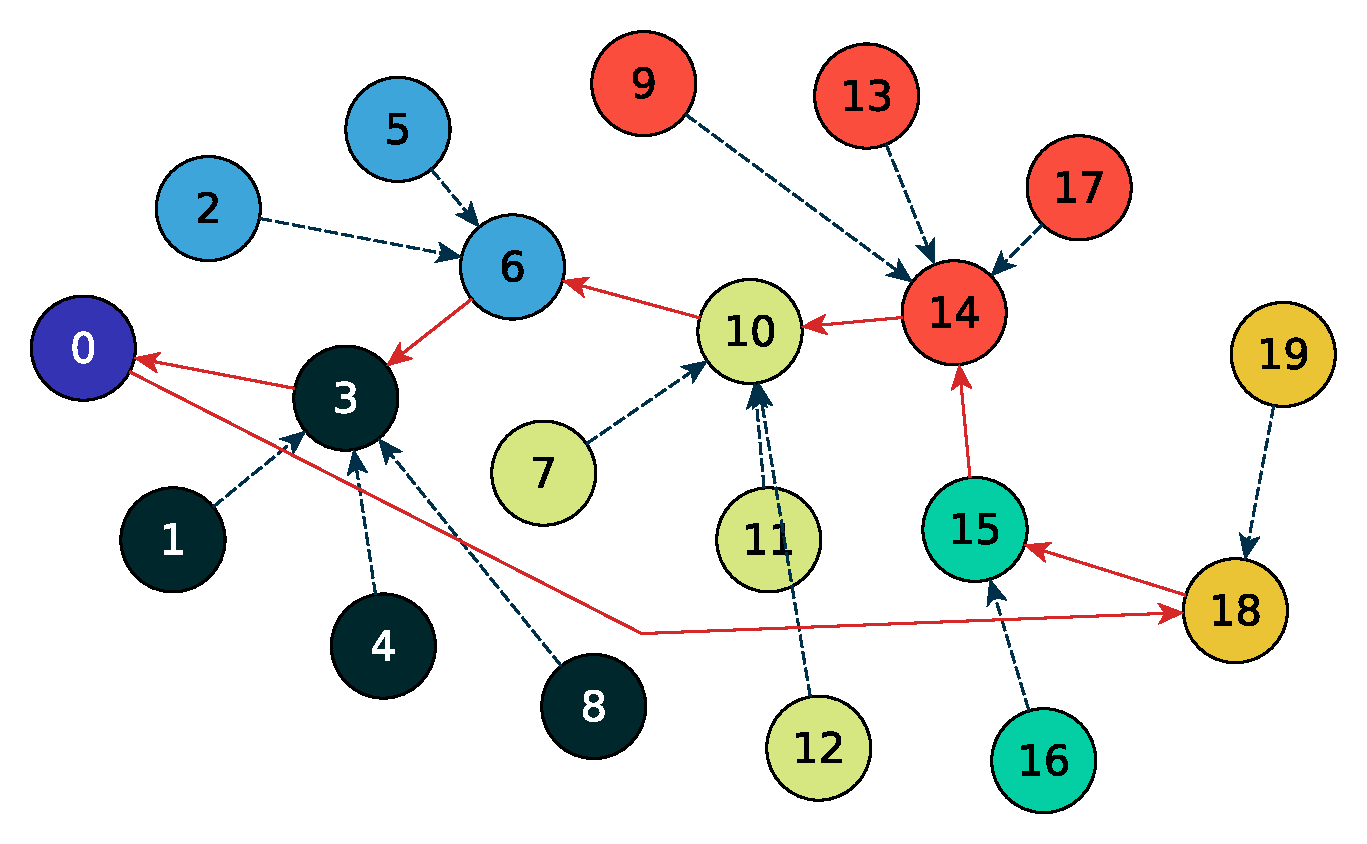
\includegraphics[width=0.4\textwidth]{images/grafo.pdf}}
\end{frame}

{\nologo
\begin{frame}
\frametitle{Results for Problem 1}
\begin{columns}
\column{0.5\textwidth}
\begin{figure}[ht]
\centering
\includegraphics[width=0.9\textwidth]{images/figure:1a.pdf}
\caption{Solutions for the cost of the tour}
\end{figure}
 
\column{0.5\textwidth}

\begin{figure}[ht]
\centering
\includegraphics[width=0.9\textwidth]{images/figure:1b.pdf}
\caption{Solutions for cumulative time}
\end{figure}
\end{columns}
\end{frame}


\begin{frame}
\frametitle{Results for Problem 1}
\begin{columns}
\column{0.5\textwidth}
\begin{figure}[ht]
\centering
\includegraphics[width=0.9\textwidth]{images/figure:2a.pdf}
\caption{GAP for the cost of the tour}
\end{figure}
 
\column{0.5\textwidth}

\begin{figure}[ht]
\centering
\includegraphics[width=0.9\textwidth]{images/figure:2b.pdf}
\caption{GAP for cumulative time}
\end{figure}
\end{columns}
\end{frame}


\begin{frame}
\frametitle{Results for Problem 1}
\begin{columns}
\column{0.5\textwidth}
\begin{figure}[ht]
\centering
\includegraphics[width=0.9\textwidth]{images/figure:3.pdf}
\caption{Number of variables}
\end{figure}
 
\column{0.5\textwidth}

\begin{figure}[ht]
\centering
\includegraphics[width=0.9\textwidth]{images/figure:4.pdf}
\caption{Number of restrictions}
\end{figure}
\end{columns}
\end{frame}

\begin{frame}
\frametitle{Results for Problem 1}
\begin{columns}
\column{0.5\textwidth}
\begin{figure}[ht]
\centering
\includegraphics[width=0.9\textwidth]{images/figure:5.pdf}
\caption{Resolution times for the cost of the tour}
\end{figure}
 
\column{0.5\textwidth}

\begin{figure}[ht]
\centering
\includegraphics[width=0.9\textwidth]{images/figure:6.pdf}
\caption{Number of Branch \& Bounds nodes explored}
\end{figure}
\end{columns}
\end{frame}

\begin{frame}
\frametitle{Results for Problem 1}
\begin{block}{Problem 1}
\begin{itemize}
\item The flow formulation finds feasible solutions in a greater number of instances.
\item The flow formulation presented a better GAP in the instances studied.
\item The multicommodity formulation generates good results, but requires a greater amount of memory
\item The multicommodity formulation finds solutions without exploring the Branch \& Bound tree
\end{itemize}
\end{block}
\end{frame}

\subsection{Results for Problem 2}
\begin{frame}
\frametitle{Results}
  \begin{beamercolorbox}[sep=8pt,center,shadow=true,rounded=true]{title}
    \usebeamerfont{title}{\LARGE Results for Problem 2}
  \end{beamercolorbox}
  \vspace{\baselineskip}
\centering{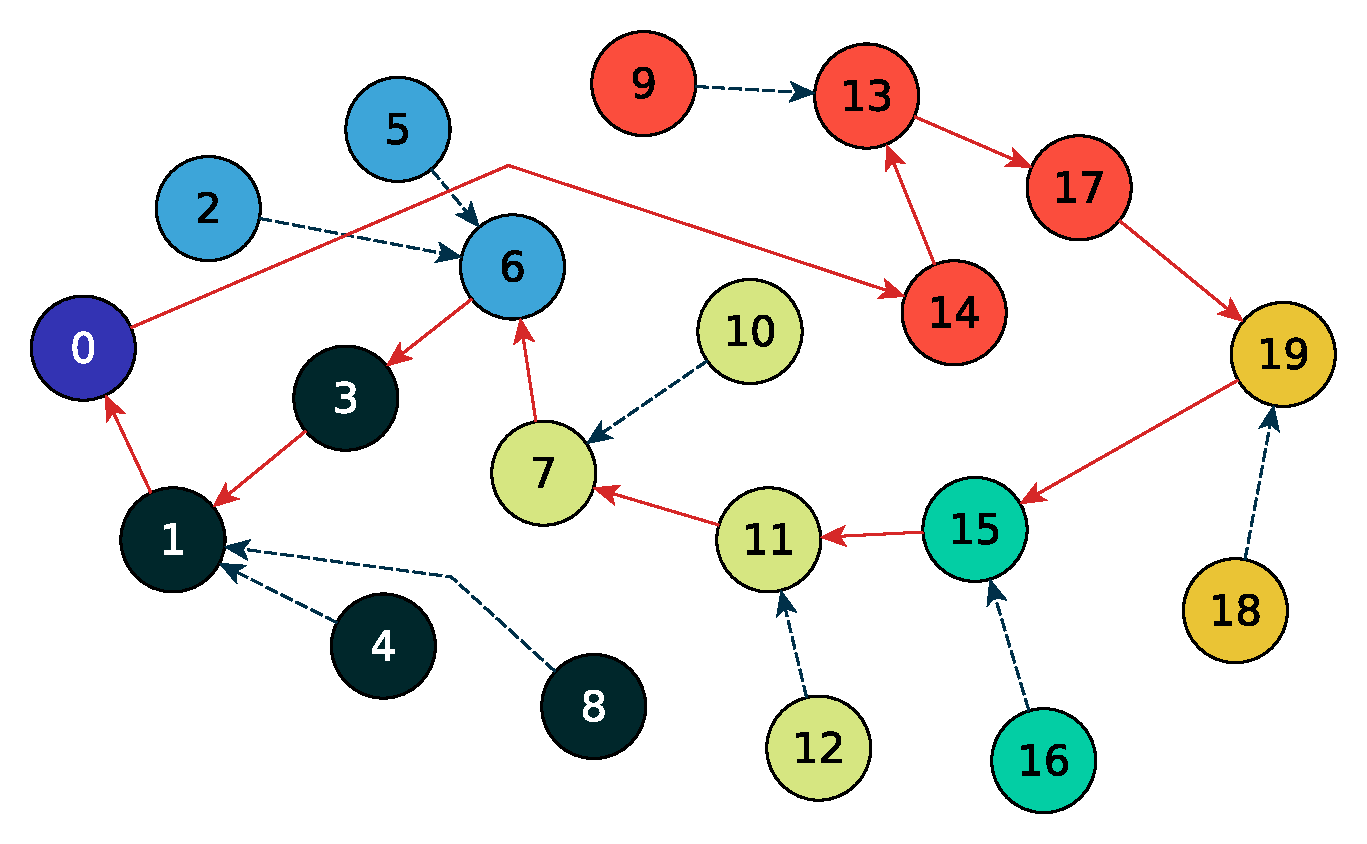
\includegraphics[width=0.4\textwidth]{images/grafo:p2.pdf}}
\end{frame}

\begin{frame}
\frametitle{Results for Problem 2}
\begin{center}
{\large The $\epsilon$-constraints method was used to find the efficient frontier:}
\end{center}

\begin{equation*}
Z_2 = \sum_{(i,j) \in A} t_{ij}^1 y_{ij} + \sum_{k \in N}\sum_{(i,j) \in A: i \neq k} t_{ij}^2  f_{ij}^k + \sum_{p = 1}^{m} \sum_{(k,j) \in \delta^+(C_{p})} t_{kj}^2 f_{kj}^k + \sum_{p = 1}^{m} \sum_{i,j \in C_p: i \neq j} t_{ij}^2 x_{ij} 
\end{equation*}
\centering{$\Downarrow$}
\begin{equation}
Z_2 \leq T_{max}
\end{equation}
\end{frame}

\begin{frame}
\frametitle{Results for Problem 2}
\begin{columns}
\column{0.5\textwidth}
\begin{figure}[ht]
\centering
\includegraphics[width=0.9\textwidth]{images/efficient-frontier:1.pdf}
\caption{Efficient frontier for burma14}
\end{figure}
 
\column{0.5\textwidth}

\begin{figure}[ht]
\centering
\includegraphics[width=0.9\textwidth]{images/efficient-frontier:2.pdf}
\caption{Efficient frontier for ulysses16}
\end{figure}
\end{columns}
\end{frame}


\begin{frame}
\frametitle{Results for Problem 2}

\begin{figure}[ht]
\centering
\includegraphics[width=0.45\textwidth]{images/efficient-frontier:3.pdf}
\caption{Efficient frontier for ulysses22}
\end{figure}
\end{frame}
}


\section[Conclusions]{Conclusions}
\begin{frame}
\frametitle{Conclusions}
\begin{itemize}
\item The proposed problem allows modeling situations where a balance between cost and quality of service is sought.
\item The proposed models are valid tools to support decision making in logistics contexts.
\item More efficient solution methods are needed to solve large instances
\end{itemize}


\end{frame}

\begin{frame}
\frametitle{Acknowledgment}
\begin{columns}
\column{0.6\textwidth}
\begin{itemize}
\item Logistics and Transport Research group - Universidad del Bío-Bío
\item Industrial Engineering Department - Universidad del Bío-Bío
\item Industrial Engineering MSc program - Universidad del Bío-Bío
\end{itemize}
\column{0.4\textwidth}
\includegraphics[width=0.5\textwidth]{logos/escudo_ubb_2}

\includegraphics[width=0.5\textwidth]{logos/DII}

\includegraphics[width=0.5\textwidth]{logos/logo-mii}
\end{columns}
\end{frame}

\begin{frame}[allowframebreaks]
\frametitle{References}
\begin{tiny}
{\tiny \bibliography{bibliography/bibliography}}
\end{tiny}


\end{frame}

\frame{\titlepage}
\frame{\frametitle{}{\tiny \color{white}
\cite{Arias-Rojas:2012}
\cite{Bektas:2007}
\cite{Current:1994}
\cite{Fischetti:1993}
\cite{Heilporn:2010}
\cite{Hillier:2010}
\cite{Jozefowiez:2007}
\cite{Jozefowiez:2008}
\cite{Kedad:2010}
\cite{Labbe:1999}
\cite{Labbe:2004}
\cite{Lari:2008}
\cite{Azimi:2012}
\cite{Ngueveu:2010}
\cite{Paredes:2009}
\cite{Park:2010}
\cite{Ribeiro:2012}
\cite{Talbi:2009}
}}

\end{document}
